%
% Categorifying the zx-calculus
% The zx-calculus
% arXiv v2
%

\documentclass[./1--Catfying_zxCalc--Master.tex]{subfiles} % ./mainfilename.tex

%%%%%%%%%%%%%%%%%%
%%%%%%%%%%%%%%%%%%
\begin{document}
%%%%%%%%%%%%%%%%%%
%%%%%%%%%%%%%%%%%%


%%%%%%%%%%%%%%%%%%%%%%
% THE ZX-CALCULUS
\section{The zx-calculus}
\label{sec:ZxCalc}
%%%%%%%%%%%%%%%%%%%%%%

One of the most fascinating features 
of quantum physics is the 
incompatibility of observables. 
Roughly, an observable is a 
measurable quantity of some system, 
for instance the spin of a photon.  
Incompatibility is in stark contrast 
to classical physics where
measurable quantities are compatible
in that, we can obtain
arbitrarily precise values 
at the same time.   
Arguably, the most famous example 
of incompatibility is 
Heisenberg's uncertainty principal
which places limits to 
the precision that one 
can simultaneously measure a 
pair of observables: 
position and momentum.  
There are different levels of 
incompatibility amongst 
pairs of observables. 
When such a pair is 
maximally incompatible, 
meaning that 
knowing one with complete precision 
implies total uncertainty of the other, 
we say they are 
\emph{complementary observables}.  

Hilbert spaces are, historically, 
the typical framework 
in which one might 
study observables.  
This formalism has been
quite successful
despite involving difficult calculations
and non-intuitive notation. 

The zx-calculus was 
developed by Coecke and Duncan 
	\cite{CoeckeDuncan_QuantumObsFullPaper} 
as a high-level language 
to facilitate such computation
between complementary observables.  
It was immediately used to 
generalize both \emph{quantum circuits}
	\cite{NielsenChuang_QuantumCompInfo}  
and the \emph{measurement calculus}
	\cite{DanosKashefiPanang_MeasurementCalc}. 
Its validity was further justified 
when Duncan and Perdrix 
presented a non-trivial method 
of verifying measurement-based 
quantum computations
	\cite{DuncanPerdrix_RewritingQuantumCompu}.  
At its core, the zx-calculus is 
an intuitive graphical language 
in which to reason about 
complementary observables. 

The five \emph{basic diagrams} 
in the zx-calculus are depicted 
in Figure \ref{fig:ZX generators}
and are to be read from left to right. 
They are
\begin{itemize}
	\item a \emph{wire} with 
		a single input and output,
	\item \emph{green spiders} with 
		a non-negative integer number of 
		inputs and outputs and 
		paired with a phase $\alpha \in [-\pi,\pi)$,
	\item \emph{red spiders} with 
		a non-negative integer number 
		inputs and outputs and 
		paired with a phase $\beta \in [-\pi,\pi)$,
	\item the \emph{Hadamard node} with
		 a single input and output, and
	\item a \emph{diamond node} with 
		no inputs or outputs.
\end{itemize}
The wire plays the role 
of an identity, much like a 
plain wire in an electrical circuit, 
or straight pipe in a plumbing system. 
The green and red spiders 
arise from a pair of 
complementary observables.  
Incredibly, observables 
correspond to certain 
commutative Frobenius algebras $A$ 
living in a 
dagger symmetric monoidal category 
	$\mathbf{C}$. 
Moreover, a pair of 
complementary observables gives a 
pair of Frobenius algebras whose 
operations interact via laws like 
those of a Hopf algebra 
	\cite{CoeckePavlovic_QuanMeasSums, 
		CoeckePavVicary_OrthogBases}.  
This is particularly nice because 
Frobenius algebras have 
beautiful string diagram representations. 
If $I$ is the monoidal unit of $\mathbf{C}$, 
there is an isomorphism 
	$\mathbf{C}(I,A) \to \mathbf{C}(A,A)$ 
of commutative monoids 
that gives rise to a 
group structure on $A$ 
known as the \emph{phase group}.  
The spider phases arise from this group.
The Hadamard node embodies 
the Hadamard gate. 
The diamond is a scalar obtained when
connecting a green and red node together.  
A deeper exploration of these notions 
goes beyond the scope of this paper.  
For those interested, 
the original paper on the topic
	\cite{CoeckeDuncan_QuantumObsFullPaper}
is an excellent place read more.

In the spirit of compositionality, 
we present a category 
$\mathbf{zx}$ below 
whose morphisms are 
generated by the 
five basic diagrams. 
To anticipate the shift
in terminology, we will
refer to zx-calculus diagrams
as \emph{$\mathbf{zx}$-morphisms} 
and continue to use the
qualifier `\emph{basic}' in the 
same way.

Observe that there is a
non-negative number of 
wires dangling on the
left and right side of each
basic $\mathbf{zx}$-morphism. 
Those on the left, 
we call \emph{inputs} 
and those on the right \emph{outputs}. 
These basic $\mathbf{zx}$-morphisms
generate the morphisms of a
dagger compact category $\mathbf{zx}$
whose objects are the non-negative integers.
This category was introduced 
by Coecke and Duncan 
	\cite{CoeckeDuncan_QuantumObsFullPaper} 
and further studied by Backens 
	\cite{Backens_Completeness}. 
To compose in $\mathbf{zx}$, 
connect compatible diagrams 
along an enumeration of the
the inputs and the outputs. 
A monoidal structure
is given by adding numbers and 
taking the disjoint union of $\mathbf{zx}$-morphisms. 
Relations between the morphisms are
given below, but we note here that
the wire is the identity on $1$.
The identity on $n$ is 
the disjoint union of $n$ wires. 
The symmetry and compactness 
of the monoidal product provide 
a braiding, evaluation, and coevaluation morphisms:
respectively,
\[

\includegraphics{InclGrphx--morphism--zx_braiding}
\quad \quad \quad \quad 
\raisebox{-0.25\height}{%
	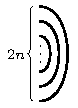
\includegraphics[scale=0.75]{InclGrphx--morphism--zx_evaluation}
}
\quad \quad \quad \quad 
\raisebox{-0.25\height}{%
	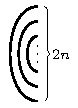
\includegraphics[scale=0.75]{InclGrphx--morphism--zx_coevaluation}
}
\]
The evaluation and coevalutation maps 
are of type 
	$2n \to 0$ and $0 \to 2n$ 
for each object $n \geq 1$ and 
the empty diagram for $n=0$.  
On the spider diagrams, 
the dagger structure 
swapps inputs and outputs then, 
multiplies the phase by $-1$:
\[
	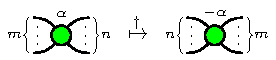
\includegraphics{InclGrphx--functor--dagger}
\]
The dagger acts trivially on the 
wire, Hadamard, and diamond elements. 

\begin{figure}
	\fbox{
		\begin{minipage}{\textwidth}
			\centering
			%%%%%%%%%%%%%%%%%%%%%%
			\subcaptionbox{Spider}{%
				\centering
				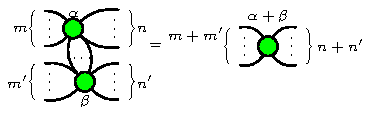
\includegraphics{InclGrphx--equation--spider}
			}
			\quad \quad
			\subcaptionbox{Bialgebra equation}{%
				\centering
				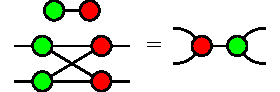
\includegraphics{InclGrphx--equation--bialgebra}
			}
			\vspace{1em} 
			\linebreak
			%%%%%%%%%%%%%%%%%%%%%%
			\subcaptionbox{Copy equation}{%
				\centering
				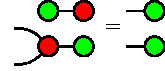
\includegraphics{InclGrphx--equation--copy}
			}
			\quad \quad 
			\subcaptionbox{$\pi$-Copy equation}{%
				\centering
				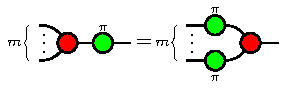
\includegraphics{InclGrphx--equation--pi_copy}
			}
			\quad \quad 
			\subcaptionbox{Cup equation}[2.5cm]{%
				\centering
				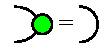
\includegraphics{InclGrphx--equation--cup}
			}
			\vspace{1em} 
			\linebreak
			%%%%%%%%%%%%%%%%%%%%%%
			\subcaptionbox{Trivial spider equation}[4cm]{%
				\centering
				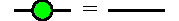
\includegraphics{InclGrphx--equation--trivial_spider}
			}
			\quad \quad \quad \quad \quad \quad 
			\subcaptionbox{$\pi$-Commutation equation}{%
				\centering
				
\includegraphics{InclGrphx--equation--pi_commutation}
			}
			\vspace{1em} 
			\linebreak
			%%%%%%%%%%%%%%%%%%%%%%
			\subcaptionbox{Color change equation}{%
				\centering
				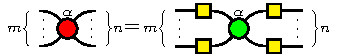
\includegraphics{InclGrphx--equation--color_change}
			}
			\subcaptionbox{Loop equation}[2.5cm]{%
				\centering
				
\includegraphics{InclGrphx--equation--loop}
			}
			\subcaptionbox{Diamond equation}[3.5cm]{%
				\centering
				
\includegraphics{InclGrphx--equation--diamond}
			}
			%%%%%%%%%%%%%%%%%%%%%%
		\end{minipage}
	}
	\caption{Relations in the category $\mathbf{zx}$}
	\label{fig:ZX equations}
\end{figure}

Thus far, we have a 
presentation for a 
free dagger compact category. 
However, there are relations 
between $\mathbf{zx}$-morphisms.
These are given in Figure \ref{fig:ZX equations},  
though we also include equations obtained by 
exchanging red and green nodes, 
daggering, and 
taking diagrams up to 
ambient isotopy in $4$-space. 
These listed relations are called \emph{basic}.  
Spiders with no phase indicated 
have a phase of $0$. 
The emergence of these relations 
goes beyond the scope of this paper
and we point the interested reader to
the genesis of the zx-calculus 
	\cite{CoeckeDuncan_QuantumObsFullPaper}
for an explanation.

A major advantage 
of using string diagrams, 
apart from their intuitive nature, 
is that computations are 
more easily programmed into 
computers.  
Indeed, graphical proof assistants
like Quantomatic 
	\cite{BarKissingerVicary_Globular,
		DixonDuncanKissinger_QuantomaticWebsite} 
and Globular 
	\cite{BarKissingerVicary_Globular} 
were tailor made for such 
graphical reasoning.  
The logic of these programs are 
encapsulated by 
double pushout rewrite rules.  
However, 
the algebraic structure of $\mathbf{zx}$ 
and other graphical calculi 
do not contain the rewrite rules 
as explicit elements.  
Perhaps, 
conceiving of rewrite rules 
as actual elements
in the syntax can prove
beneficial for software programmers.

%%%%%%%%%%%%%%%%%%
%%%%%%%%%%%%%%%%%%
% 
\end{document}
%
%%%%%%%%%%%%%%%%%%
%%%%%%%%%%%%%%%%%%
